\chapter{Introduction}
Javascript is growing rapid fast in mobile web development, server architectures, rest services, desktop cross plattform apps and microservices with the help of nodejs. On top of that every developer can choose which frontend platform is the best choice. React is developed by facebook and provides dynamic DOM manipulation without the need of reloading the complete DOM on every change.

Beside that react has a huge community base for additional custom components and active issue tracking. Definitely something you should keep an eye on.

\section{Structure}
Every react component follows the same structure. Define your needed imports of react base code and additional components you want your component to use.

Define the default export name and what exactly should be exported. Normally it is your component for sure. A simple code example could look like this:

\begin{lstlisting}
import React, { Component, PropTypes } from 'react'
import { Paper, RaisedButton, TextField } from 'material-ui'

export default class TestName extends Component {
	render() {
		return (
			<Paper style={{ width: 300 }}>
				<TextField
					hintText="Benutzername"
					style={{ float: 'left' }}
				/>
				<TextField
					hintText="Passwort"
					style={{ float: 'middle' }}
				/>
				<RaisedButton
					label="Login"
					style={{ float: 'right' }}
				/>
			</Paper>
		)
	}
}
\end{lstlisting}

\section{UI}
The rendered code above will look like this:
  \begin{figure}[htb!]
	\centerline{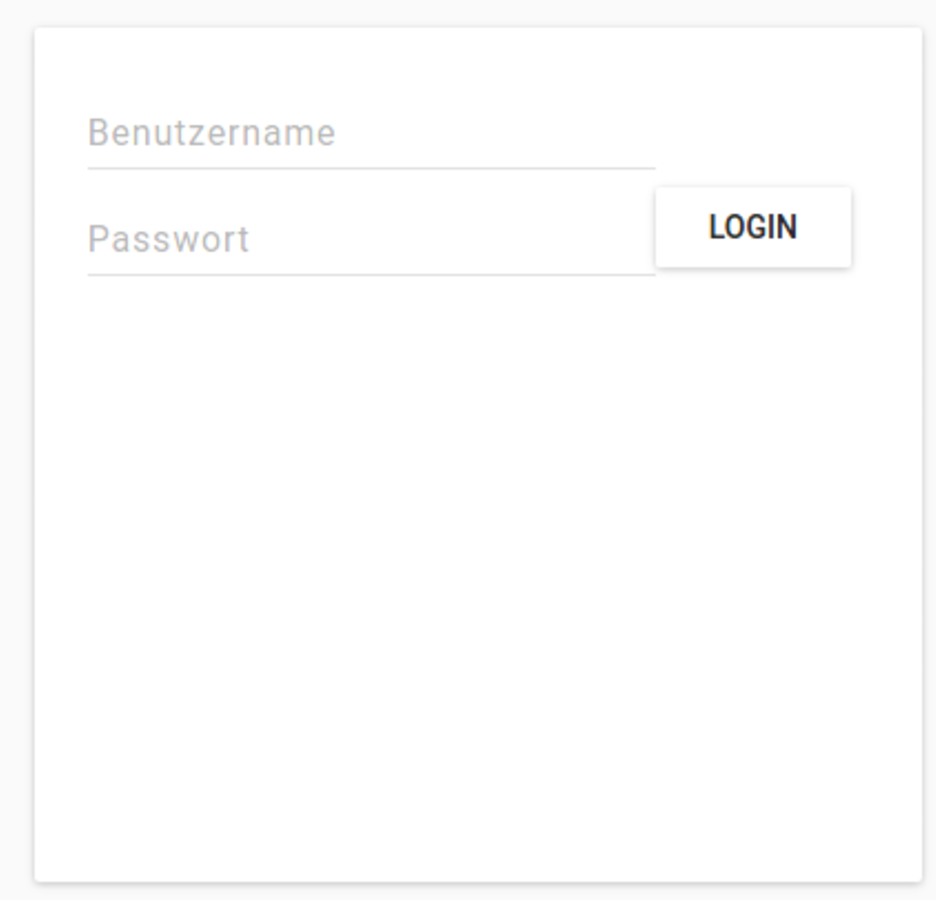
\includegraphics[width=0.8\textwidth]{resources/preview.png}}
\end{figure}